\documentclass[tikz,12pt,border=2pt]{standalone}
\usepackage[T1]{fontenc}
\usepackage[scaled=0.92]{helvet}
\renewcommand{\familydefault}{\sfdefault}
\usetikzlibrary{arrows.meta,positioning}
\definecolor{accent}{RGB}{31,84,140}
\definecolor{accentlight}{RGB}{200,214,232}
\begin{document}
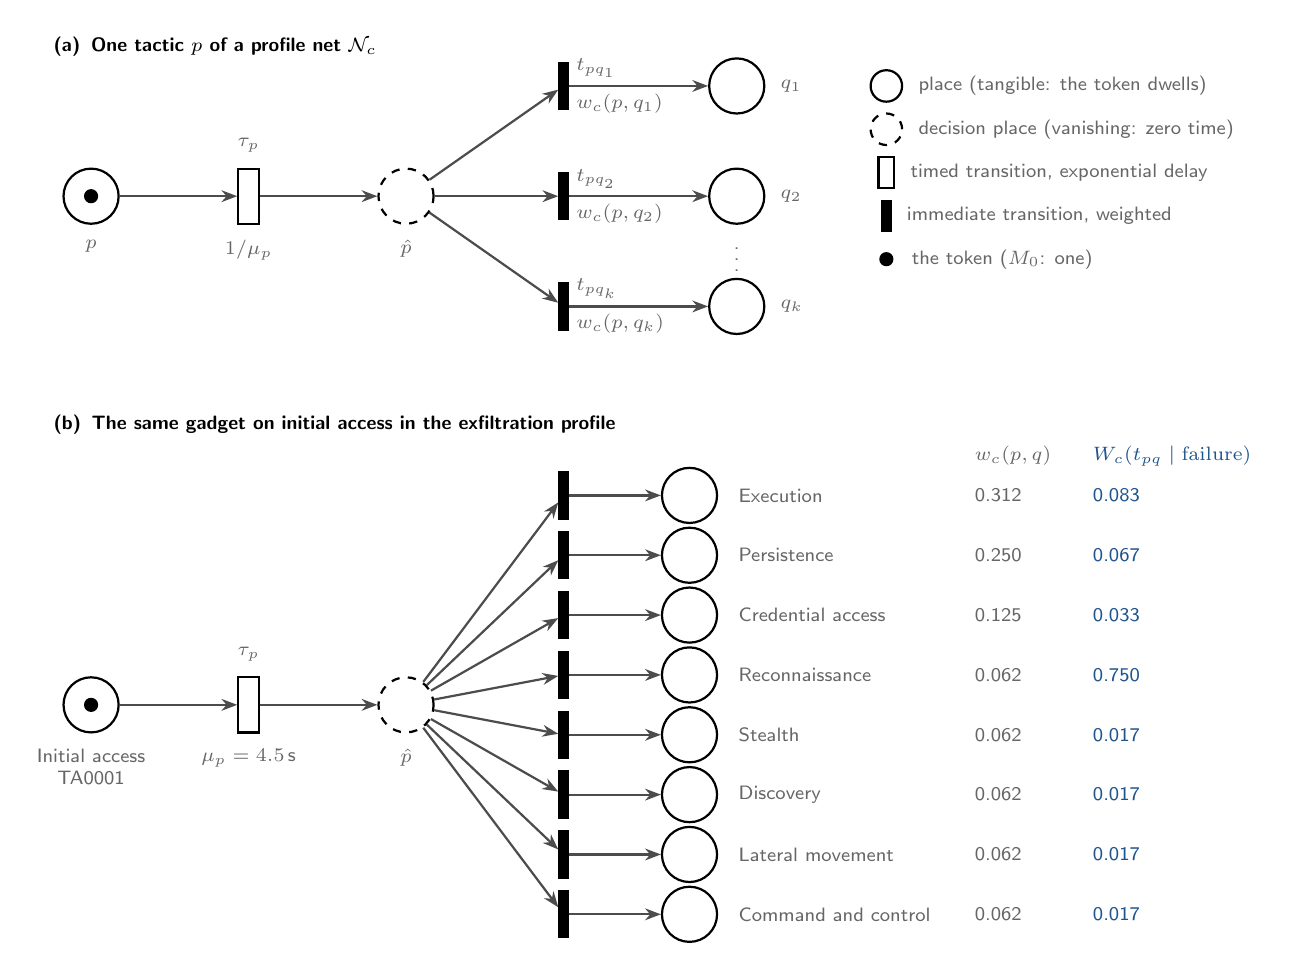
\begin{tikzpicture}[
  font=\scriptsize,
  place/.style={circle,draw=black,thick,minimum size=7mm,inner sep=0pt},
  vplace/.style={circle,draw=black,thick,dashed,minimum size=7mm,inner sep=0pt},
  timed/.style={rectangle,draw=black,thick,fill=white,minimum width=2.6mm,minimum height=7mm,inner sep=0pt},
  imm/.style={rectangle,draw=black,fill=black,minimum width=1.2mm,minimum height=6mm,inner sep=0pt},
  arc/.style={-{Stealth[length=2mm]},thick,black!70},
  lab/.style={black!60,font=\scriptsize},
  head/.style={font=\scriptsize\bfseries},
]
\node[head,anchor=west] at (-0.6,3.4) {(a)\enspace One tactic $p$ of a profile net $\mathcal{N}_c$};
\node[place] (p) at (0.0,1.5) {}; \fill (p) circle (0.9mm);
\node[below=2pt of p,lab,align=center] {$p$};
\node[timed] (tau) at (2.0,1.5) {};
\node[above=2pt of tau,lab] {$\tau_p$};
\node[below=2pt of tau,lab] {$1/\mu_p$};
\node[vplace] (ph) at (4.0,1.5) {};
\node[below=2pt of ph,lab] {$\hat{p}$};
\draw[arc] (p) -- (tau); \draw[arc] (tau) -- (ph);
\node[imm] (t1) at (6.0,2.9) {};
\node[place] (q1) at (8.2,2.9) {};
\node[right=2pt of q1,lab] {$q_1$};
\draw[arc] (ph) -- (t1); \draw[arc] (t1) -- (q1);
\node[lab,anchor=south west,inner sep=1pt] at (6.12,2.96) {$t_{pq_1}$};
\node[lab,anchor=north west,inner sep=1pt] at (6.12,2.84) {$w_c(p,q_1)$};
\node[imm] (t2) at (6.0,1.5) {};
\node[place] (q2) at (8.2,1.5) {};
\node[right=2pt of q2,lab] {$q_2$};
\draw[arc] (ph) -- (t2); \draw[arc] (t2) -- (q2);
\node[lab,anchor=south west,inner sep=1pt] at (6.12,1.56) {$t_{pq_2}$};
\node[lab,anchor=north west,inner sep=1pt] at (6.12,1.44) {$w_c(p,q_2)$};
\node[imm] (t3) at (6.0,0.10000000000000009) {};
\node[place] (q3) at (8.2,0.10000000000000009) {};
\node[right=2pt of q3,lab] {$q_k$};
\draw[arc] (ph) -- (t3); \draw[arc] (t3) -- (q3);
\node[lab,anchor=south west,inner sep=1pt] at (6.12,0.1600000000000001) {$t_{pq_k}$};
\node[lab,anchor=north west,inner sep=1pt] at (6.12,0.04000000000000009) {$w_c(p,q_k)$};
\node[lab] at (8.2,0.8) {$\vdots$};
\node[place,minimum size=4mm] (lp) at (10.1,2.9) {}; \node[right=2pt of lp,lab] {place (tangible: the token dwells)};
\node[vplace,minimum size=4mm] (lv) at (10.1,2.3499999999999996) {}; \node[right=2pt of lv,lab] {decision place (vanishing: zero time)};
\node[timed,minimum height=4mm,minimum width=2mm] (lt) at (10.1,1.7999999999999998) {}; \node[right=2pt of lt,lab] {timed transition, exponential delay};
\node[imm,minimum height=4mm] (li) at (10.1,1.25) {}; \node[right=2pt of li,lab] {immediate transition, weighted};
\fill (10.1,0.6999999999999997) circle (0.9mm); \node[lab,anchor=west] at (10.299999999999999,0.6999999999999997) {the token ($M_0$: one)};
\node[head,anchor=west] at (-0.6,-1.4) {(b)\enspace The same gadget on \emph{initial access} in the exfiltration profile};
\node[place] (bp) at (0.0,-4.96) {}; \fill (bp) circle (0.9mm);
\node[below=2pt of bp,lab,align=center] {Initial access\\TA0001};
\node[timed] (btau) at (2.0,-4.96) {};
\node[above=2pt of btau,lab] {$\tau_p$};
\node[below=2pt of btau,lab] {$\mu_p = 4.5$\,s};
\node[vplace] (bph) at (4.0,-4.96) {};
\node[below=2pt of bph,lab] {$\hat{p}$};
\draw[arc] (bp) -- (btau); \draw[arc] (btau) -- (bph);
\node[lab,anchor=west] at (11.1,-1.7999999999999998) {$w_c(p,q)$};
\node[lab,anchor=west,accent] at (12.6,-1.7999999999999998) {$W_c(t_{pq}\mid\mathrm{failure})$};
\node[imm] (bt1) at (6.0,-2.3) {};
\node[place] (bq1) at (7.6,-2.3) {};
\node[lab,anchor=west] at (8.1,-2.3) {Execution};
\node[lab,anchor=west] at (11.1,-2.3) {0.312};
\node[lab,anchor=west,accent] at (12.6,-2.3) {0.083};
\draw[arc] (bph) -- (bt1); \draw[arc] (bt1) -- (bq1);
\node[imm] (bt2) at (6.0,-3.0599999999999996) {};
\node[place] (bq2) at (7.6,-3.0599999999999996) {};
\node[lab,anchor=west] at (8.1,-3.0599999999999996) {Persistence};
\node[lab,anchor=west] at (11.1,-3.0599999999999996) {0.250};
\node[lab,anchor=west,accent] at (12.6,-3.0599999999999996) {0.067};
\draw[arc] (bph) -- (bt2); \draw[arc] (bt2) -- (bq2);
\node[imm] (bt3) at (6.0,-3.82) {};
\node[place] (bq3) at (7.6,-3.82) {};
\node[lab,anchor=west] at (8.1,-3.82) {Credential access};
\node[lab,anchor=west] at (11.1,-3.82) {0.125};
\node[lab,anchor=west,accent] at (12.6,-3.82) {0.033};
\draw[arc] (bph) -- (bt3); \draw[arc] (bt3) -- (bq3);
\node[imm] (bt4) at (6.0,-4.58) {};
\node[place] (bq4) at (7.6,-4.58) {};
\node[lab,anchor=west] at (8.1,-4.58) {Reconnaissance};
\node[lab,anchor=west] at (11.1,-4.58) {0.062};
\node[lab,anchor=west,accent] at (12.6,-4.58) {0.750};
\draw[arc] (bph) -- (bt4); \draw[arc] (bt4) -- (bq4);
\node[imm] (bt5) at (6.0,-5.34) {};
\node[place] (bq5) at (7.6,-5.34) {};
\node[lab,anchor=west] at (8.1,-5.34) {Stealth};
\node[lab,anchor=west] at (11.1,-5.34) {0.062};
\node[lab,anchor=west,accent] at (12.6,-5.34) {0.017};
\draw[arc] (bph) -- (bt5); \draw[arc] (bt5) -- (bq5);
\node[imm] (bt6) at (6.0,-6.1) {};
\node[place] (bq6) at (7.6,-6.1) {};
\node[lab,anchor=west] at (8.1,-6.1) {Discovery};
\node[lab,anchor=west] at (11.1,-6.1) {0.062};
\node[lab,anchor=west,accent] at (12.6,-6.1) {0.017};
\draw[arc] (bph) -- (bt6); \draw[arc] (bt6) -- (bq6);
\node[imm] (bt7) at (6.0,-6.86) {};
\node[place] (bq7) at (7.6,-6.86) {};
\node[lab,anchor=west] at (8.1,-6.86) {Lateral movement};
\node[lab,anchor=west] at (11.1,-6.86) {0.062};
\node[lab,anchor=west,accent] at (12.6,-6.86) {0.017};
\draw[arc] (bph) -- (bt7); \draw[arc] (bt7) -- (bq7);
\node[imm] (bt8) at (6.0,-7.62) {};
\node[place] (bq8) at (7.6,-7.62) {};
\node[lab,anchor=west] at (8.1,-7.62) {Command and control};
\node[lab,anchor=west] at (11.1,-7.62) {0.062};
\node[lab,anchor=west,accent] at (12.6,-7.62) {0.017};
\draw[arc] (bph) -- (bt8); \draw[arc] (bt8) -- (bq8);
\end{tikzpicture}
\end{document}
